\begin{problem}{Japanese Game}{standard input}{standard output}{3 seconds}{512 megabytes}

Joseph really likes the culture of Japan. Last year he learned Japanese traditional clothes and visual arts and now he is trying to find out the secret of the Japanese game called Nonogram.

In the one-dimensional version of the game, there is a row of $n$ empty cells, some of which are to be filled with a pen. There is a description of a solution called a \emph{profile}~--- a sequence of positive integers denoting the lengths of consecutive sets of filled cells. For example, the profile of $[4, 3, 1]$ means that there are sets of four, three, and one filled cell, in that order, with at least one empty cell between successive sets.

\begin{center}
\includegraphics[scale=1]{001.eps}

A suitable solution for $n = 12$ and $p = [4, 3, 1]$.
\end{center}

\begin{center}
\includegraphics[scale=1]{002.eps}

A wrong solution: the first four filled cells should be consecutive.
\end{center}

\begin{center}
\includegraphics[scale=1]{003.eps}

A wrong solution: there should be at least one empty cell before the last filled cell.
\end{center}

Joseph found out that for some numbers $n$ and profiles $p$ there are lots of ways to fill the cells to satisfy the profile. Now he is in the process of solving a nonogram consisting of $n$ cells and a profile $p$. He has already created a \emph{mask} of $p$~--- he has filled all the cells that must be filled in every solution of the nonogram.

\begin{center}
\includegraphics[scale=1]{004.eps}

The mask for $n = 12$ and $p = [4, 3, 1]$: all the filled cells above are filled in every solution.
\end{center}

After a break, he lost the source profile $p$. He only has $n$ and the mask $m$. Help Joseph find any profile $p'$ with the mask $m$ or say that there is no such profile and Joseph has made a mistake.

\InputFile
The only line contains a string $m$~--- the mask of the source profile $p$.
The length of $m$ is $n$ ($1 \le n \le 100\,000$).
The string $m$ consists of symbols \texttt{\#} and \texttt{\_}~--- denoting filled and empty cells respectively.


\OutputFile
If there is no profile with the mask $m$, output the number $-1$.
Otherwise, on the first line, output an integer $k$~--- the number of integers in the profile $p'$. 
On the second line, output $k$ integers of the profile $p'$.

\Examples

\begin{example}
\exmpfile{example.01}{example.01.a}%
\exmpfile{example.02}{example.02.a}%
\exmpfile{example.03}{example.03.a}%
\end{example}

\end{problem}

